\begin{figure}
  \centering
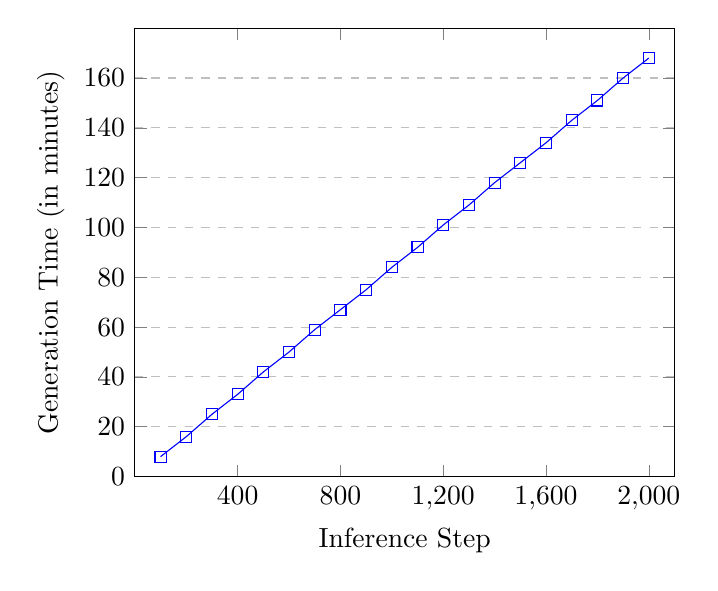
\begin{tikzpicture}
\begin{axis}[
    xlabel={Inference Step},
    ylabel={Generation Time (in minutes)},
    xmin=0, xmax=2100,
    ymin=0, ymax=180,
    xtick={400,800,1200,1600,2000},
    ytick={0,20,40,60,80,100,120,140,160},
    ymajorgrids=true,
    grid style=dashed,
]

\addplot[
    color=blue,
    mark=square,
    ]
    coordinates {
    (100,8)(200,16)(300,25)(400,33)(500,42)(600,50)(700,59)(800,67)(900,75)(1000,84)(1100,92)(1200,101)(1300,109)(1400,118)(1500,126)(1600,134)(1700,143)(1800,151)(1900,160)(2000,168)
    };
    
\end{axis}
\end{tikzpicture}
% 扩散模型生成128张大小为128*128的图片所用的时间。
  \caption{The time taken by the diffusion model to generate 128 images of size 128x128.}
  \label{fig:generate_time}
\end{figure}